\chapter{Design and Implementation}
\label{chap:design-implementation}

% ------------------------------------------------------------------ styles
\usetikzlibrary{positioning,calc,fit,decorations.pathreplacing}
\definecolor{hostc}{HTML}{DCE8F5}
\definecolor{devc}{HTML}{FBE3C8}
\definecolor{memc}{HTML}{DDF0DA}
\definecolor{padc}{HTML}{D9D9D9}
\definecolor{lA}{HTML}{8DB6E0}
\definecolor{lB}{HTML}{F2B880}
\definecolor{lC}{HTML}{9CCF95}
\definecolor{lD}{HTML}{E59A9A}
\definecolor{lE}{HTML}{C3A7DB}
\definecolor{lF}{HTML}{E8D98A}
\tikzset{
  dbox/.style={draw,rounded corners=2pt,align=center,font=\small,inner sep=4pt,fill=devc},
  hbox/.style={draw,rounded corners=2pt,align=center,font=\small,inner sep=4pt,fill=hostc},
  mbox/.style={draw,rounded corners=2pt,align=center,font=\small,inner sep=4pt,fill=memc},
  darr/.style={-{Latex[length=2mm]},thick},
  sectag/.style={font=\sffamily\scriptsize,fill=white,draw=gray,rounded corners=1pt,inner sep=1.5pt},
}


\section{System Architecture}
\label{sec:system-architecture}
This chapter presents the system design and implementation of a Tenstorrent-oriented IVF-Flat approximate nearest-neighbor search pipeline on a single-chip Tenstorrent Wormhole n150 device using TT-Metalium \cite{tenstorrent_metalium_architecture,tenstorrent_wormhole_spec}. IVF-Flat provides the underlying indexing algorithm; the contribution of this chapter is its mapping to the target accelerator. In particular, the design maps regular, fixed-shape operations, including centroid scoring and page-wise candidate scoring, onto the tile-oriented Tensix execution model, while explicitly handling the irregularity caused by query-dependent list selection and unequal inverted-list sizes; the choice of IVF-Flat itself is motivated in Section~\ref{sec:index-suitability}.

The implementation is organized around two principal device programs: a \emph{coarse-search program}, which compares queries with the IVF centroids, and a \emph{fine-search program}, which evaluates candidate vectors from the selected inverted lists and reduces the results to the final top-\(k\). Host-side processing connects the two phases by selecting the \(N_{\mathrm{probe}}\) lists returned by coarse search and constructing the work schedule used by the fine-search workers. Figure~\ref{fig:design-map} gives an overview of the complete search; the tag on each step indicates the section of this chapter that describes it.

\begin{figure}[htbp]
\centering
\resizebox{\textwidth}{!}{%
\begin{tikzpicture}[font=\small]
\fill[hostc!40] (-0.4,0.9) rectangle (16.0,3.6);
\fill[devc!45] (-0.4,-3.6) rectangle (16.0,0.5);
\node[anchor=west,font=\bfseries\small] at (-0.3,3.3) {Host CPU};
\node[anchor=west,font=\bfseries\small] at (-0.3,-3.35) {Tenstorrent device};
\draw[dashed,gray] (-0.4,0.7) -- (16.0,0.7);
\node[font=\scriptsize,gray,fill=white,inner sep=1pt] at (12.0,0.7) {PCIe};
% host
\node[hbox,minimum width=2.6cm,minimum height=1.1cm] (load) at (1.2,2.0)
  {Build index,\\upload once};
\node[sectag,anchor=south east] at (load.north east) {\S\ref{sec:device-oriented-ivf}};
\node[hbox,minimum width=2.6cm,minimum height=1.1cm] (launch) at (4.4,2.0)
  {Upload queries,\\launch coarse};
\node[sectag,anchor=south east] at (launch.north east) {\S\ref{sec:coarse-search}};
\node[hbox,minimum width=3.6cm,minimum height=1.1cm] (sched) at (8.9,2.0)
  {Select \(N_{\mathrm{probe}}\) lists,\\schedule them on workers};
\node[sectag,anchor=south east] at (sched.north east) {\S\ref{sec:fine-search-scheduling}};
\node[hbox,minimum width=1.8cm,minimum height=1.1cm] (out) at (14.9,2.0)
  {Read result,\\keep \(k\)};
\node[sectag,anchor=south east] at (out.north east) {\S\ref{subsec:hierarchical-topk}};
% device
\node[mbox,minimum width=2.3cm,minimum height=1.1cm] (dram) at (1.2,-1.9)
  {Index in DRAM\\(pages + IDs)};
\node[sectag,anchor=south east] at (dram.north east) {\S\ref{subsec:tiled-list-layout}};
\node[dbox,minimum width=2.6cm,minimum height=1.1cm] (coarse) at (5.3,-1.9)
  {Coarse\\search};
\node[sectag,anchor=south] at (coarse.north) {\S\ref{sec:coarse-search}};
\node[dbox,minimum width=3.0cm,minimum height=1.1cm] (fine) at (8.9,-1.9)
  {Fine search on\\63 workers};
\node[sectag,anchor=south east] at (fine.north east) {\S\ref{subsec:fine-worker-pipeline}};
\node[dbox,minimum width=2.4cm,minimum height=1.1cm] (agg) at (12.9,-1.9)
  {Final top-32 on\\core \((0,0)\)};
\node[sectag,anchor=south east] at (agg.north east) {\S\ref{subsec:hierarchical-topk}};
% arrows
\draw[darr] (load) -- (dram);
\draw[darr] (dram) -- node[above,font=\scriptsize]{centroids} (coarse);
\draw[darr] (4.6,1.45) -- node[pos=0.5,left,font=\scriptsize]{queries} (4.6,-1.35);
\draw[darr] (6.0,-1.35) -- node[pos=0.5,right,font=\scriptsize,align=left]{top-32 lists\\per query} (6.0,0.0) -| (7.6,1.45);
\draw[darr] (sched.south) -- node[pos=0.55,right,font=\scriptsize,align=left]{list tasks\\per worker} (fine.north);
\draw[darr] (dram.south) -- (1.2,-3.0) -| node[pos=0.25,below,font=\scriptsize]{pages of the selected lists} (8.9,-2.45);
\draw[darr] (fine) -- node[above,font=\scriptsize,align=center]{partial\\top-32} (agg);
\draw[darr] (agg.north) |- node[pos=0.25,right,font=\scriptsize]{final top-32} (out.west);
\node[font=\scriptsize,anchor=east] at (15.9,-3.3)
  {All batches of a workload: one invocation (\S\ref{sec:multi-batch-execution})};
\end{tikzpicture}}
\caption{Map of the chapter. Host steps are on top and device steps below; the
tag on each box gives the section that describes it. The index is uploaded
once; every query workload then runs through the remaining steps.}
\label{fig:design-map}
\end{figure}

\subsection{End-to-End Search Pipeline}
\label{subsec:end-to-end-pipeline}

A query is first compared with all \(N_{\mathrm{list}}\) centroids, after which the \(N_{\mathrm{probe}}\) most similar centroids identify the inverted lists to be searched. Candidate vectors contained in those lists are then compared with the query, and the final top-\(k\) scores and vector identifiers are selected from the resulting similarities.


The selected candidates are not copied into a single temporary matrix. Instead, database vectors remain grouped by inverted list in device memory and are streamed directly from the selected lists during fine search.

Queries are represented internally in groups containing between one and 32 valid queries, matching the row dimension of the \(32\times32\) tile representation used by the Tensix compute kernels. A group containing fewer than 32 valid queries is completed with zero-valued padded rows. For a workload containing \(Q\) valid queries, the implementation uses
\begin{equation}
B=\left\lceil\frac{Q}{32}\right\rceil
\end{equation}
internal query batches. The final batch is padded when \(Q\) is not divisible by 32. The number of valid rows is retained separately, so padded rows do not participate in coarse-result processing and do not contribute inverted lists to the fine-search schedule. They are also discarded when the final results are converted back to the host representation.

Although the implementation is described throughout the chapter in terms of one 32-query batch for clarity, the final system can process multiple such batches within one coarse-search and one fine-search invocation. The transition from the initial single-batch implementation to this multi-batch design is discussed in Section~\ref{sec:multi-batch-execution}.

\subsection{Host--Device Work Partitioning}
\label{subsec:host-device-responsibilities}

The index data required by both search stages remain resident on the Tenstorrent device across query workloads, including the centroid matrix, database vectors grouped by inverted list, and the corresponding original vector identifiers. In contrast, query-dependent data, such as the query buffer, coarse-search outputs, selected-list metadata, worker schedules, partial results, and final outputs, are updated for each search workload.

A synchronization boundary separates the coarse and fine programs. After the device executes coarse search and returns a fixed-size set of centroid candidates for each valid query, the host performs the final \(N_{\mathrm{probe}}\) selection, obtains the offset and padded length of each corresponding inverted list, groups the selected work at batch granularity, and constructs the per-worker fine-search descriptions. Only once this query-dependent schedule has been prepared is the fine-search program launched.

The selection of the \(N_{\mathrm{probe}}\) lists and the steps that follow it run on the host rather than on the device because they require a set-like, dynamically sized data structure. The lists selected by the up to 32 queries of a batch must be collected into a set without duplicates, whose size depends on how much the selections overlap, and the resulting lists must then be split into chunks, sorted by size, and distributed among the workers. Such structures fit the Tensix cores poorly: each core has only a limited amount of L1 memory, which the search already uses for its circular buffers, and the programming model is built around fixed-size tiles and streams rather than dynamically growing containers (Section~\ref{sec:tt-architecture}). On the host, the same work is simple and cheap: it takes 7.8--10.7~ms per 10,000 queries at \(N_{\mathrm{list}}=512\), at most 3\% of the search time (Section~\ref{sec:tt-stage-results}).

The division of responsibilities between the host and the device corresponds to the two rows of Figure~\ref{fig:design-map}, and the synchronization boundary to the arrows that cross the PCIe line between them.


Each device program is decomposed into \emph{reader}, \emph{compute}, and \emph{writer} kernels connected through circular buffers, allowing data movement and computation to overlap when dependencies and buffer capacity permit it. Throughout this chapter, reader, compute, and writer denote kernels executing on a Tensix core, whereas worker and aggregation core denote logical roles assigned to complete Tensix cores.

\subsection{Running Example}
\label{subsec:running-example}

To make the following sections easier to follow, all examples in this chapter use the same small configuration. It keeps the structure of the real search but replaces every size with a small one, so that each step can be drawn in full. Table~\ref{tab:running-example} lists the example values next to the real ones. The eight example lists A--H hold 7, 3, 10, 4, 5, 2, 6, and 3 vectors, and the four queries of the batch select the lists \(q_0\):~\{A,~C\}, \(q_1\):~\{A,~B\}, \(q_2\):~\{C,~E\}, and \(q_3\):~\{A,~D\}; lists F, G, and H are selected by no query.

\begin{table}[htbp]
\centering
\small
\caption{Sizes in the running example and in the real implementation.}
\label{tab:running-example}
\begin{tabular}{lcc}
\toprule
& Example & Real implementation \\
\midrule
Tile size & \(4\times4\) & \(32\times32\) \\
Queries per batch & 4 (\(q_0\)--\(q_3\)) & 32 \\
Vector dimensions (padded) & 3 (4) & 100 (128) \\
Vectors per page & 4 & 32 \\
Inverted lists \(N_{\mathrm{list}}\) & 8 (A--H) & 512--2048 \\
Lists per query \(N_{\mathrm{probe}}\) & 2 & 1--32 \\
Top-\(k\) state per query & top-2 & top-32 \\
Results returned per query & 2 & \(k\le32\) (\(k=10\) evaluated) \\
Fine-search workers & 3 (W1--W3) & 63 \\
Chunk limit & 2 pages & 128 pages \\
\bottomrule
\end{tabular}
\end{table}

\section{Device-Oriented IVF Representation}
\label{sec:device-oriented-ivf}

\subsection{Index Construction}
\label{subsec:index-construction}

Index training is treated as an offline preprocessing step and is outside the timed search path. The training split is clustered with Faiss \(k\)-means, using its default settings, which sample at most 256 training vectors per centroid, to obtain \(N_{\mathrm{list}}\) centroids \cite{faiss}, following the same training procedure used by the CPU and GPU baselines based on Faiss \texttt{IndexIVFScalarQuantizer} with \texttt{QT\_fp16} storage. The trained centroid matrix is exported and reused by the Tenstorrent implementation. Reusing the same centroids avoids making index-training quality an additional experimental variable and allows the evaluation to focus on differences in search execution.

Training is not performed on the Tenstorrent device because the objective of this work is the online IVF search path rather than accelerator-based \(k\)-means. An on-device training implementation would require additional iterative kernels for vector assignment, per-cluster accumulation, centroid normalization, and convergence control, together with temporary device-memory capacity for the intermediate state. Those operations would neither be part of the measured query path nor improve the fairness of the search comparison. During construction of the Tenstorrent-oriented index, each database vector is assigned to its closest exported centroid and placed in the corresponding packed inverted list.

The Tenstorrent index stores full, uncompressed database vectors rather than compressed representations. Database vectors and centroids are normalized before assignment and search, allowing inner product to be used as the similarity measure.

\subsection{Tiled Data Layout and Memory Placement}
\label{subsec:tiled-list-layout}

As introduced in Chapter~\ref{chap:background}, Tensix computation is organized around \(32\times32\) tiles \cite{tenstorrent_metalium_architecture}. Let \(D\) denote the original vector dimension. To match this tile-oriented execution model, the dimension is padded to
\begin{equation}
D_{\mathrm{p}}=32\left\lceil\frac{D}{32}\right\rceil.
\label{eq:dimension-padding}
\end{equation}
All values introduced by dimensional padding are set to zero on the host before the data are transferred to the device.

Vectors assigned to the same inverted list are stored consecutively in one logical packed database buffer. For a list containing \(L_j\) valid vectors, its stored length is rounded to a multiple of 32:
\begin{equation}
L_{j,\mathrm{p}}=32\left\lceil\frac{L_j}{32}\right\rceil.
\label{eq:list-padding}
\end{equation}
Each group of 32 vectors forms one \emph{candidate page}. A page contains \(D_{\mathrm{p}}/32\) 16-bit floating-point (\texttt{FP16}) data tiles, each of shape \(32\times32\), which together represent the 32 candidate vectors over the complete padded dimension. Centroids and queries use the same \texttt{FP16} representation, while vector identifiers are stored as 32-bit unsigned integers (\texttt{UInt32}). The Tenstorrent compute configuration enables FP32 destination accumulation. In this implementation, this is not merely a numerical-precision choice but a compatibility requirement of the employed top-\(k\) kernel path, which applies the score ordering to companion \texttt{UInt32} identifier tiles.

A candidate page must not be confused with a query batch. A query batch contains up to 32 queries and forms the row operand of fine search, whereas a candidate page contains 32 database vectors and forms the column operand. Their matrix product evaluates every query in the batch against every vector in the page. Figure~\ref{fig:pedagogical-batch-page} illustrates this distinction with the \(4\times4\) tiles of the running example.

\begin{figure}[htbp]
\centering
\resizebox{0.98\textwidth}{!}{%
\begin{tikzpicture}[font=\small]
\node[draw,rounded corners,fill=blue!8,inner sep=7pt] (queries) {$
Q_b=
\begin{bmatrix}
q_0^{\mathsf T}\\
q_1^{\mathsf T}\\
q_2^{\mathsf T}\\
q_3^{\mathsf T}
\end{bmatrix}_{4\times D_{\mathrm p}}
$};
\node[draw,rounded corners,fill=green!9,inner sep=7pt,
      right=1.2cm of queries] (page) {$
V_p=
\begin{bmatrix}
\vert&\vert&\vert&\vert\\[-2pt]
v_0&v_1&v_2&v_3\\[-2pt]
\vert&\vert&\vert&\vert
\end{bmatrix}_{D_{\mathrm p}\times4}
$};
\node[draw,rounded corners,fill=orange!12,inner sep=7pt,
      right=1.2cm of page] (scores) {$
S_{b,p}=
\begin{bmatrix}
s_{00}&s_{01}&s_{02}&s_{03}\\
s_{10}&s_{11}&s_{12}&s_{13}\\
s_{20}&s_{21}&s_{22}&s_{23}\\
s_{30}&s_{31}&s_{32}&s_{33}
\end{bmatrix}
$};
\node at ($(queries.east)!0.5!(page.west)$) {$\times$};
\node at ($(page.east)!0.5!(scores.west)$) {$=$};
\node[below=3pt of queries,font=\scriptsize] {query batch};
\node[below=3pt of page,font=\scriptsize] {candidate page};
\node[below=3pt of scores,font=\scriptsize] {query--candidate scores};
\end{tikzpicture}
}
\caption{\(4\times4\) example of one fine-search matrix
multiplication. Rows represent queries and columns represent candidate vectors.
The implementation uses \(32\times32\) tiles rather than the reduced size
shown here.}
\label{fig:pedagogical-batch-page}
\end{figure}

For every candidate page, one full \(32\times32\) \texttt{UInt32} identifier tile is stored. In its DRAM representation, each column corresponds to one candidate vector and the same 32 identifiers are replicated across all query rows. For candidate identifiers \(i_0,\ldots,i_{31}\), the stored tile is
\begin{equation}
I^{\mathrm{stored}}=
\begin{bmatrix}
i_0 & i_1 & \cdots & i_{31}\\
i_0 & i_1 & \cdots & i_{31}\\
\vdots & \vdots & \ddots & \vdots\\
i_0 & i_1 & \cdots & i_{31}
\end{bmatrix}.
\label{eq:identifier-tile}
\end{equation}
Before the compute-kernel \texttt{topk\_local\_sort} operation, both the similarity tile and its companion identifier tile are transposed. The identifier tile presented to the selection operation is therefore
\begin{equation}
I^{\mathrm{topk}}
=
\left(I^{\mathrm{stored}}\right)^{\mathsf T}
=
\begin{bmatrix}
i_0 & i_0 & \cdots & i_0\\
i_1 & i_1 & \cdots & i_1\\
\vdots & \vdots & \ddots & \vdots\\
i_{31} & i_{31} & \cdots & i_{31}
\end{bmatrix}.
\label{eq:identifier-tile-topk}
\end{equation}
After transposition, each column corresponds to one query and the rows represent candidate entries. The \texttt{topk\_local\_sort} operation sorts candidate entries independently for each query column. Applying the same transpose and ordering operations to the score and identifier tiles preserves the association between every similarity value and its original database-vector identifier. The same mechanism updates every running top-32 state in coarse and fine search (Section~\ref{subsec:fine-worker-pipeline}).

Identifiers are stored as complete tiles because data are fetched from DRAM and processed by the compute engines in units of tiles, and \texttt{topk\_local\_sort} requires a full identifier tile next to the score tile. The cost is that a 4,096-byte identifier tile accompanies every 8,192-byte page of vectors, so one third of the bytes read by fine search are identifiers.

The vectors of all inverted lists are stored sequentially in a single packed device buffer. Each inverted list is identified by its offset within this buffer and by its length, rather than being stored in a separate device allocation. Vector identifiers occupy a separate packed \texttt{UInt32} buffer using the same list and page ordering. An inverted-list offset therefore identifies a position in this global logical representation. At the physical memory level, TT-Metalium interleaves buffer pages across DRAM banks, so ``contiguous'' refers to the logical buffer layout rather than to consecutive bytes within one DRAM bank.

Figure~\ref{fig:example-layout} shows this layout for the running example. List A holds 7 vectors and therefore occupies two pages, the second with one padded slot; list C holds 10 vectors in three pages and is longer than the example chunk limit of two pages, so it is later scheduled as two tasks (Section~\ref{subsec:greedy-work-distribution}).

\begin{figure}[htbp]
\centering
\resizebox{\textwidth}{!}{%
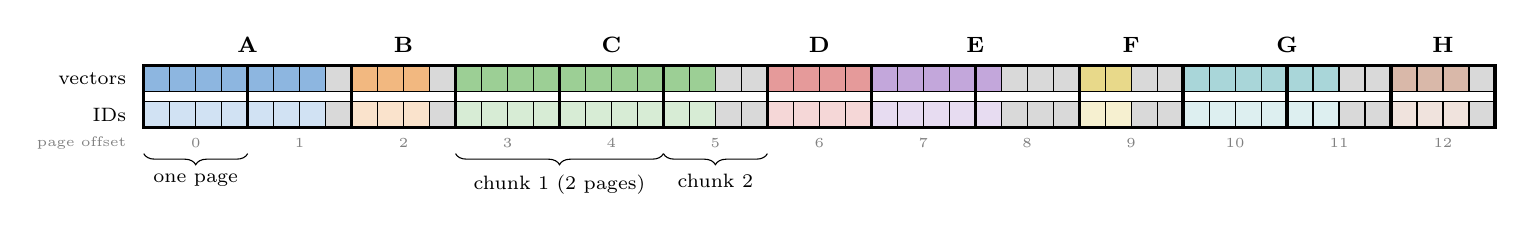
\begin{tikzpicture}[x=3.3mm,y=3.3mm]
\definecolor{lG}{HTML}{A9D6D9}\definecolor{lH}{HTML}{D9B8A9}
\foreach \name/\valid/\slots/\col/\start in
  {A/7/8/lA/0, B/3/4/lB/8, C/10/12/lC/12, D/4/4/lD/24, E/5/8/lE/28, F/2/4/lF/36, G/6/8/lG/40, H/3/4/lH/48}{
  \foreach \i in {1,...,\slots}{
    \pgfmathsetmacro{\xx}{\start+\i-1}
    \ifnum\i>\valid
      \draw[fill=padc] (\xx,0) rectangle ++(1,1);
      \draw[fill=padc] (\xx,-1.4) rectangle ++(1,1);
      \node[font=\tiny] at (\xx+0.5,-0.9) {\(\varnothing\)};
    \else
      \draw[fill=\col] (\xx,0) rectangle ++(1,1);
      \draw[fill=\col!40] (\xx,-1.4) rectangle ++(1,1);
    \fi
  }
  \node[font=\footnotesize\bfseries] at (\start+\slots/2,1.8) {\name};
  \pgfmathtruncatemacro{\np}{\slots/4}
  \foreach \p in {1,...,\np}{\draw[very thick] (\start+4*\p-4,-1.4) rectangle ++(4,2.4);}
}
\foreach \o in {0,...,12}{\node[font=\tiny,gray] at (4*\o+2,-2.0) {\o};}
\node[anchor=east,font=\tiny,gray] at (-0.3,-2.0) {page offset};
\node[anchor=east,font=\scriptsize] at (-0.3,0.5) {vectors};
\node[anchor=east,font=\scriptsize] at (-0.3,-0.9) {IDs};
\draw[decorate,decoration={brace,mirror,amplitude=4pt}] (0,-2.4) -- (4,-2.4)
  node[midway,below=4pt,font=\scriptsize] {one page};
\draw[decorate,decoration={brace,mirror,amplitude=4pt}] (12,-2.4) -- (20,-2.4)
  node[midway,below=4pt,font=\scriptsize] {chunk 1 (2 pages)};
\draw[decorate,decoration={brace,mirror,amplitude=4pt}] (20,-2.4) -- (24,-2.4)
  node[midway,below=4pt,font=\scriptsize] {chunk 2};
\end{tikzpicture}}
\caption{Packed layout of the example index in device DRAM. Each thick box is
one page of 4 vectors with its identifier tile (one row of it is drawn; the
stored tile repeats this row for every query row), and the numbers below give
the page offsets. Gray slots are list padding carrying the sentinel identifier
\(\varnothing\). List C exceeds the chunk limit of 2 pages and is scheduled as
two chunks.}
\label{fig:example-layout}
\end{figure}

Persistent search data are allocated in device DRAM, including the centroid matrix, packed database-vector buffer, and packed vector-identifier buffer. Query buffers and worker descriptions are likewise allocated in DRAM for each search workload, while per-core L1 memory is used as transient kernel-local storage through circular buffers. During execution, data required by the active kernels are streamed from DRAM into L1 rather than persistently cached across search invocations. The exact reuse and streaming strategy of the coarse- and fine-search programs is described in Sections~\ref{sec:coarse-search} and~\ref{subsec:fine-worker-pipeline}, respectively.

Padding is performed entirely on the host before device transfer:
\begin{itemize}
    \item database dimensional padding and inverted-list length padding are generated during \texttt{IVF\_TT::create\_index};
    \item centroid dimensional padding is generated while constructing the centroid buffer in \texttt{load\_to\_device};
    \item query dimensional padding and final-batch row padding are generated in \texttt{search\_all}.
\end{itemize}
Padded vector identifiers are assigned the sentinel value \texttt{0xffffffff} on the host.

Padded candidate positions contain zero-valued vectors and carry the sentinel identifiers defined above. Because the kernel also knows the size of every list it processes, it recognizes the last page of a list and, if that page is partially populated, linearly scans its score and identifier entries before the top-\(k\) update. Whenever a sentinel identifier is encountered, the corresponding similarity value is replaced with \(-10000\), preventing padded candidates from displacing valid results during selection. The database and query vectors are normalized, so a valid inner product is bounded below by \(-1\) in exact arithmetic; \(-10000\) is therefore safely outside the valid similarity range. Complete candidate pages contain 32 valid vectors and bypass this masking step, avoiding an unnecessary scan of all \(32\times32=1024\) entries when no padding is present.

\section{Coarse Search}
\label{sec:coarse-search}

The purpose of coarse search is to identify the inverted lists most relevant to each query. For a valid query batch \(Q_b\in\mathbb{R}^{32\times D_{\mathrm{p}}}\) and centroid matrix \(C\in\mathbb{R}^{D_{\mathrm{p}}\times N_{\mathrm{list}}}\), the logical operation is
\begin{equation}
S^{\mathrm{coarse}}_b=Q_bC,
\label{eq:coarse-search}
\end{equation}
where each row of \(S^{\mathrm{coarse}}_b\) contains the similarities between one query and all centroids.

Tiling proceeds over blocks of 32 centroids. After loading the query batch from DRAM into an L1 circular buffer, the reader kernel streams centroid blocks from device DRAM while retaining the query tiles for reuse across the complete centroid matrix. Let \(C_c\in\mathbb{R}^{D_{\mathrm{p}}\times32}\) denote centroid block \(c\).

The corresponding coarse-similarity tile is
\begin{equation}
S^{\mathrm{coarse}}_{b,c}=Q_bC_c,
\qquad
S^{\mathrm{coarse}}_{b,c}\in\mathbb{R}^{32\times32}.
\label{eq:coarse-similarity-tile}
\end{equation}
Rather than materializing all \(N_{\mathrm{list}}\) similarities in DRAM, the compute kernel incrementally maintains the 32 highest centroid scores and their identifiers for each query row. This running top-32 state uses the same transpose-and-\texttt{topk\_local\_sort} mechanism described in Section~\ref{subsec:tiled-list-layout}, with identical ordering decisions applied to scores and centroid identifiers.

Figure~\ref{fig:example-coarse} shows coarse search for the running example. The query tile is multiplied with the eight centroids in two blocks of four, and after each block the best two lists of every query are updated. After the first block, \(q_2\) holds C (0.9) and D (0.3); in the second block, E scores 0.8 and replaces D, so the final selection of \(q_2\) is \{C,~E\}. The other queries keep their first-block selections, since no list of the second block beats them.

\begin{figure}[htbp]
\centering
\resizebox{0.95\textwidth}{!}{%
\begin{tikzpicture}[x=5mm,y=5mm,font=\scriptsize]
\foreach \r in {0,...,3}{\foreach \c in {0,...,3}{
  \ifnum\c=3 \def\f{padc}\else\def\f{hostc}\fi
  \draw[fill=\f] (\c,-\r) rectangle ++(1,1);}
  \node[anchor=east] at (-0.1,-\r+0.5) {\(q_{\r}\)};}
\node[font=\small] at (2,1.8) {\(Q\) (4 queries)};
\node at (5,-1) {\(\times\)};
\foreach \r in {0,...,3}{\foreach \c in {0,...,3}{
  \ifnum\r=3 \def\f{padc}\else\def\f{memc}\fi
  \draw[fill=\f] (6+\c,-\r) rectangle ++(1,1);}}
\foreach \c/\n in {0/A,1/B,2/C,3/D}{\node at (6.5+\c,1.5) {\n};}
\node[font=\small] at (8,2.6) {centroid block 1};
\node at (11,-1) {\(=\)};
\foreach \r in {0,...,3}{\foreach \c in {0,...,3}{\draw[fill=devc] (12+\c,-\r) rectangle ++(1,1);}}
\foreach \r/\a/\b/\c/\d in {0/.9/.2/.7/.1, 1/.8/.6/.3/.2, 2/.2/.1/.9/.3, 3/.7/.3/.2/.6}{
  \node at (12.5,-\r+0.5) {\a}; \node at (13.5,-\r+0.5) {\b};
  \node at (14.5,-\r+0.5) {\c}; \node at (15.5,-\r+0.5) {\d};}
\foreach \c/\n in {0/A,1/B,2/C,3/D}{\node at (12.5+\c,1.5) {\n};}
\node[font=\small] at (14,2.6) {scores};
\foreach \r in {0,...,3}{\foreach \c in {0,...,3}{
  \ifnum\r=3 \def\f{padc}\else\def\f{memc}\fi
  \draw[fill=\f] (6+\c,-\r-6) rectangle ++(1,1);}}
\foreach \c/\n in {0/E,1/F,2/G,3/H}{\node at (6.5+\c,-4.5) {\n};}
\node[font=\small] at (8,-3.5) {centroid block 2};
\node at (5,-7) {\(Q\,\times\)};
\node at (11,-7) {\(=\)};
\foreach \r in {0,...,3}{\foreach \c in {0,...,3}{\draw[fill=devc] (12+\c,-\r-6) rectangle ++(1,1);}}
\foreach \r/\a/\b/\c/\d in {0/.3/.4/.2/.1, 1/.1/.4/.2/.3, 2/.8/.5/.1/.2, 3/.4/.1/.3/.2}{
  \node at (12.5,-\r-5.5) {\a}; \node at (13.5,-\r-5.5) {\b};
  \node at (14.5,-\r-5.5) {\c}; \node at (15.5,-\r-5.5) {\d};}
\foreach \c/\n in {0/E,1/F,2/G,3/H}{\node at (12.5+\c,-4.5) {\n};}
\node[dbox,align=left,anchor=west] (t1) at (17.2,-1)
  {top-2 after block 1\\[2pt]
   \(q_0\): A, C\quad \(q_1\): A, B\\
   \(q_2\): C, \textbf{D}\quad \(q_3\): A, D};
\node[dbox,align=left,anchor=west] (t2) at (17.2,-7)
  {top-2 after block 2\\[2pt]
   \(q_0\): A, C\quad \(q_1\): A, B\\
   \(q_2\): C, \textbf{E}\quad \(q_3\): A, D};
\draw[darr] (16.3,-1) -- (t1.west);
\draw[darr] (16.3,-7) -- (t2.west);
\draw[darr] (t1.south) -- (t1.south|-t2.north);
\end{tikzpicture}}
\caption{Coarse search in the example. The query tile stays in L1 while the
centroid blocks are streamed from DRAM; after each block, the best two lists of
every query are updated; in the second block, E replaces D for \(q_2\). Gray
cells are dimension padding.}
\label{fig:example-coarse}
\end{figure}

Once all centroid blocks assigned to a query batch have been processed, the coarse-search writer kernel running on the same participating Tensix core writes one score tile and one identifier tile for that batch to device DRAM. After copying these results to the host, the host retains the first \(N_{\mathrm{probe}}\) centroid identifiers of each valid query. Because the queries of a batch can select the same lists, the resulting \(32\times N_{\mathrm{probe}}\) matrix of identifiers can contain the same list several times; the host removes these duplicates when it forms the batch-level union described in Section~\ref{subsec:batch-level-union}. Because the coarse search keeps a top-32 state per query, the current implementation limits \(N_{\mathrm{probe}}\) to at most 32.

The coarse-search program distributes the query batches across all available Tensix cores, with each active core processing one or more complete batches and avoiding inter-core communication during the centroid scan. Because every valid query is evaluated against the same centroid matrix, coarse search remains regular and requires a predictable amount of work.

\section{Fine-Search Scheduling}
\label{sec:fine-search-scheduling}

Fine search introduces the principal source of irregularity in the system. Every valid query selects the same number \(N_{\mathrm{probe}}\) of inverted lists, but the identifiers and lengths of those lists depend on the query. Two queries with the same \(N_{\mathrm{probe}}\) may therefore require very different amounts of candidate processing. The imbalance remains after lists are combined at batch level: one worker assigned several short lists can finish before another worker assigned one very long list.

The scheduler estimates the cost of a selected list by its number of padded 32-vector candidate pages. Lists longer than 128 pages, that is 4,096 vectors, are split into consecutive chunks of at most 128 pages, each scheduled as a separate task, while shorter lists remain a single task. The limit of 128 pages was chosen experimentally, as the value that performed best among those tested for the evaluated list sizes.

\subsection{Batch-Level List Union}
\label{subsec:batch-level-union}

After coarse search, each query row has up to \(N_{\mathrm{probe}}\) selected inverted-list identifiers. Since fine search operates on a complete batch of up to 32 queries, the host collects these identifiers into a single set of lists for the batch.

Let \(\mathcal{P}_{b,r}\) denote the \(N_{\mathrm{probe}}\) lists selected for query row \(r\) of batch \(b\). The set of lists processed for the batch is
\begin{equation}
\mathcal{U}_b
=
\bigcup_{r\in\mathcal{V}_b}
\mathcal{P}_{b,r},
\label{eq:batch-union}
\end{equation}
where \(\mathcal{V}_b\) contains the valid query rows of the batch.

Operationally, the host iterates over the coarse-search results of every valid query row and inserts the first \(N_{\mathrm{probe}}\) list identifiers into a set. Duplicate identifiers are therefore automatically removed. The resulting set \(\mathcal{U}_b\) contains every inverted list selected by at least one query in the batch.

The batch-level union follows from the execution granularity of the Tensix matrix engine. Multiplying a page \(V_p\in\mathbb{R}^{D_{\mathrm{p}}\times32}\) by the query tiles \(Q_b\in\mathbb{R}^{32\times D_{\mathrm{p}}}\) costs the same whether one or all 32 query rows need its scores, so once a page has been fetched, scoring it for every query of the batch requires no additional multiplication.

As a consequence, a query can also obtain similarity scores for vectors belonging to a list that was selected by another query in the same batch. The effective candidate set for one query can therefore be larger than the set defined by its own \(N_{\mathrm{probe}}\) lists. This is an implementation consequence of processing the batch-level union and does not modify the stored IVF index. Section~\ref{sec:nlist-nprobe-results} shows that, with queries batched in dataset order, the queries of a batch share few lists, so the union is close to \(32N_{\mathrm{probe}}\) lists and each query is scored against 12 to 32 times as many vectors as its own lists contain.

The union can nevertheless increase the total amount of fine-search work because lists selected by different queries may not overlap, increasing the number of distinct candidate pages that must be processed. The benefit of the design therefore comes from fully exploiting each tile-level matrix multiplication, rather than from making the additional lists computationally free.

\subsection{Greedy Work Distribution}
\label{subsec:greedy-work-distribution}

For each list \(j\in\mathcal{U}_b\), the host creates one task for the entire list or one task per chunk, as described above. A list \(j\) with \(L_j\) valid vectors has
\begin{equation}
n_j=\left\lceil\frac{L_j}{32}\right\rceil
\label{eq:list-scheduling-weight}
\end{equation}
padded pages; lists containing 320 and 288 vectors, for example, have 10 and 9 pages. The weight \(n_t\) of a task \(t\) is its own page count, which equals \(n_j\) for a complete list and at most 128 for a chunk, and counts the fixed-shape page multiplications the task requires.

The fine-search program uses all Tensix cores available to it, an \(8\times8\) logical grid of 64 cores. Logical core \((0,0)\) is reserved for final aggregation, and the remaining 63 cores form the fine-search worker set \(\mathcal{W}\). For every query batch, let \(\mathcal{A}_{b,w}\) denote the tasks assigned to worker \(w\). The scheduler resets both the assignments and their estimated loads,
\begin{equation}
\mathcal{A}_{b,w}=\varnothing,
\qquad
\lambda_{b,w}=0,
\qquad w\in\mathcal{W},
\end{equation}
sorts the tasks in non-increasing order of \(n_t\), and assigns each task \(t\) to a currently least-loaded worker:
\begin{align}
w^*&=\arg\min_{w\in\mathcal{W}}\lambda_{b,w},\\
\mathcal{A}_{b,w^*}&\leftarrow\mathcal{A}_{b,w^*}\cup\{t\},\\
\lambda_{b,w^*}&\leftarrow\lambda_{b,w^*}+n_t.
\label{eq:greedy-list-assignment}
\end{align}
Tasks with equal page counts are ordered by ascending list identifier, and chunks of the same list by their position in the list. If several workers have the same minimum load, the worker with the lowest index is selected. These explicit tie rules make the host schedule reproducible. The resulting longest-processing-time-first (LPT) greedy policy balances the padded page count of each batch while retaining sequential access within every packed list. Because the loads are reset for every batch, a batch with fewer tasks than workers always assigns its work to the lowest-indexed workers, and imbalances are not compensated across batches; Section~\ref{subsec:tt-device-timeline-results} shows how worker imbalance sets the batch completion time.

Figure~\ref{fig:example-schedule} shows the complete process for the running example. The four queries select eight lists, but only five are distinct, since A is shared by three queries and C by two, so \(\mathcal U_b=\{\)A, B, C, D, E\(\}\). List C has three pages, more than the example chunk limit of two, so it becomes two tasks, C\(_1\) with two pages and C\(_2\) with one. Sorted by weight and assigned to the least-loaded worker, the six tasks give each of the three workers exactly three pages. Every worker then scores all four queries against its pages, so query \(q_1\), for example, also receives scores for list C, which it did not select.

\begin{figure}[htbp]
\centering
\begin{tikzpicture}[font=\small]
\node[hbox,align=left] (sel) at (0,0)
  {\(q_0\): A, C\\ \(q_1\): A, B\\ \(q_2\): C, E\\ \(q_3\): A, D};
\node[above=1mm of sel,font=\scriptsize] {8 selections};
\node[hbox,align=left,right=10mm of sel] (uni)
  {\(\mathcal U=\{\)A, B, C, D, E\(\}\)\\[2pt]
   A: 2 pages, B: 1, C: 3,\\ D: 1, E: 2};
\node[above=1mm of uni,font=\scriptsize] {union: 5 distinct lists};
\draw[darr] (sel) -- node[above,font=\scriptsize]{dedup.} (uni);
\node[hbox,align=left,right=10mm of uni] (tasks)
  {sorted tasks:\\ A (2), C\(_1\) (2), E (2),\\ B (1), C\(_2\) (1), D (1)};
\node[above=1mm of tasks,font=\scriptsize] {C split into 2 chunks};
\draw[darr] (uni) -- (tasks);
\begin{scope}[shift={($(tasks.south)+(-1.6,-0.9)$)},x=8mm,y=6mm]
  \foreach \w/\a/\ac/\b/\bc [count=\i] in
    {W1/A/lA/B/lB, W2/C\(_1\)/lC/C\(_2\)/lC, W3/E/lE/D/lD}{
    \node[anchor=east,font=\small] at (-0.2,-\i+0.4) {\w};
    \draw[fill=\ac] (0,-\i) rectangle node{\a} (2,-\i+0.8);
    \draw[fill=\bc] (2,-\i) rectangle node{\b} (3,-\i+0.8);
  }
  \node[font=\scriptsize,anchor=west] at (3.2,-2) {3 pages each};
\end{scope}
\draw[darr] (tasks.south) -- ++(0,-0.6) node[right,font=\scriptsize]{LPT};
\end{tikzpicture}
\caption{From selections to worker tasks in the example. The union removes
duplicate lists, the long list C is split into chunks, and the tasks are
assigned longest-first to the least-loaded worker (LPT).}
\label{fig:example-schedule}
\end{figure}

The page count is an estimate rather than a cycle-accurate cost model. It does not capture per-list setup, masking of the final partial page, variation in memory service time, circular-buffer waiting, or synchronization. Moreover, because tasks remain coarse, with up to 128 pages each, the largest task can still determine the batch completion time. After scheduling, the host serializes one description per fine-search worker so that its reader kernel can locate the assigned lists and chunks in device memory.

\subsection{Worker Description}
\label{subsec:worker-description}

The host serializes the assignment of each fine-search worker into a
flattened worker description in DRAM, which may span several DRAM pages. For
\(B\) query batches (Section~\ref{subsec:end-to-end-pipeline}), the
description of worker \(w\) is
\begin{equation}
\mathcal{D}_w=\left\langle B,\,R_{w,0},\,R_{w,1},\,\ldots,\,R_{w,B-1}\right\rangle,
\label{eq:worker-description}
\end{equation}
with one record per batch,
\begin{equation}
R_{w,b}=\left\langle o^{Q}_b,\,n^{Q}_b,\,N_{w,b},\,
E_{w,b,0},\,\ldots,\,E_{w,b,N_{w,b}-1}\right\rangle,
\qquad
E_{w,b,e}=\left\langle o^{V}_{w,b,e},\,n^{V}_{w,b,e}\right\rangle.
\label{eq:worker-batch-record}
\end{equation}
Here \(o^{Q}_b\) and \(n^{Q}_b\) are the offset and tile count of query batch
\(b\) in the query buffer, and \(N_{w,b}\) is the number of tasks assigned to
worker \(w\) for that batch. Each entry \(E_{w,b,e}\) describes one task, a
complete list or a chunk, by its page offset \(o^{V}_{w,b,e}\) in the packed
database buffer and its page count \(n^{V}_{w,b,e}=n_t\). Because every page
holds 32 vectors, the offset and page count are enough for the reader to fetch
the task's vector and identifier tiles. In the running example, where the pages of lists A to H occupy the packed offsets 0--1, 2, 3--5, 6, 7--8, 9, 10--11, and 12 (Figure~\ref{fig:example-layout}), the single batch record of each worker is
\begin{center}
\small
W1: \(\langle 0,1,2,\ \langle0,2\rangle,\langle2,1\rangle\rangle\)\qquad
W2: \(\langle 0,1,2,\ \langle3,2\rangle,\langle5,1\rangle\rangle\)\qquad
W3: \(\langle 0,1,2,\ \langle7,2\rangle,\langle6,1\rangle\rangle\),
\end{center}
that is, query offset 0, one query tile, two tasks, and one offset--count pair per task.

At the start of fine search, each worker copies its description into L1. For
every batch with assigned work, the reader loads the query tiles once into the
query circular buffer, where they stay while all tasks of that batch are
processed, and then moves to the next batch record.

\section{Fine Search and Result Reduction}
\label{sec:fine-search-and-reduction}

\subsection{Worker Pipeline}
\label{subsec:fine-worker-pipeline}

Each of the 63 fine-search workers executes reader, compute, and writer kernels concurrently, working through its description as described in Section~\ref{subsec:worker-description}. Figure~\ref{fig:data-movement} shows where data move during the search and how the RISC-V cores of one Tensix core share the work of a worker: the NCRISC core runs the reader, the three TRISC cores run the unpack, math, and pack stages of the compute kernel, and the BRISC core runs the writer.

\begin{figure}[htbp]
\centering
\resizebox{\textwidth}{!}{%
\begin{tikzpicture}[font=\small]
\node[hbox,minimum width=2.0cm,minimum height=1.2cm] (host) at (0,0.4) {Host\\memory};
\node[mbox,minimum width=3.0cm,minimum height=4.8cm] (dram) at (4.2,0.4)
  {Device DRAM\\[2pt]\scriptsize 12\,GB GDDR6,\\\scriptsize 6 controllers,\\\scriptsize 12 channels\\[4pt]\scriptsize index pages + IDs,\\\scriptsize queries, worker\\\scriptsize descriptions,\\\scriptsize partial results};
\draw[darr,<->] (host) -- node[above,font=\scriptsize]{PCIe} (dram);
\draw[rounded corners=3pt,fill=devc!35] (8.6,-0.45) rectangle (15.6,3.0);
\node[anchor=north west,font=\small\bfseries] at (8.7,2.95) {worker core (\(\times\)63)};
\node[dbox,minimum width=2.4cm] (rd) at (10.3,1.75) {reader\\\scriptsize NCRISC};
\node[dbox,minimum width=2.8cm] (cp) at (13.8,1.75) {compute\\\scriptsize TRISC0--2: unpack,\\\scriptsize math, pack};
\node[dbox,minimum width=2.4cm] (wr) at (10.3,0.45) {writer\\\scriptsize BRISC};
\draw[darr] (rd) -- node[above,font=\scriptsize]{CBs} (cp);
\draw[darr] (cp.south) |- (wr.east);
\node[font=\scriptsize,anchor=west] at (8.7,-0.2) {L1: query tiles, 2 page + ID slots, top-32 state};
\node[dbox,minimum width=7.0cm,minimum height=0.9cm] (agg) at (12.1,-1.55)
  {\textbf{aggregation core} \((0,0)\)};
\draw[darr] (5.7,1.75) -- node[above,font=\scriptsize]{pages over NoC} (rd.west);
\draw[darr] (wr.west) -- node[above,font=\scriptsize]{partial top-32} (5.7,0.45);
\draw[darr] (5.7,-1.3) -- node[above,font=\scriptsize]{gather} (agg.west|-0,-1.3);
\draw[darr] (agg.west|-0,-1.8) -- node[below,font=\scriptsize]{final top-32} (5.7,-1.8);
\end{tikzpicture}}
\caption{Data movement during the search and roles of the RISC-V cores of a
worker. The index is uploaded once; for each workload, the queries are written
to device DRAM, and every worker streams its pages over the network-on-chip
(NoC) into L1 circular buffers (CBs). The reader, compute, and writer kernels
run on different RISC-V cores, so the next page can be read while the current
one is scored. The partial results reach the aggregation core through DRAM.}
\label{fig:data-movement}
\end{figure}

Candidate vectors and their identifier tiles are streamed from the packed DRAM buffers. The reader issues both reads before a shared synchronization barrier, allowing their transfers over the on-device Network-on-Chip (NoC) to be outstanding concurrently. Double-buffering of the candidate circular buffers allows the reader to prepare a later page while the compute kernel operates on an earlier one, subject to circular-buffer capacity and producer--consumer synchronization.

The candidate-data and candidate-identifier circular buffers provide two alternating slot pairs. After the reader fills slot pair~0 with page \(p\), the compute kernel can consume that page while the reader fills slot pair~1 with page \(p+1\). Once compute releases slot pair~0, the reader can reuse it for page \(p+2\) while compute consumes slot pair~1. This pipelining can hide part of the page-read cost, although the achieved overlap remains subject to NoC completion, circular-buffer availability, and relative reader and compute progress.


Let \(t\) identify a task assigned to the worker and \(p\) a page within it. For one such page \(V_{t,p}\in\mathbb{R}^{D_{\mathrm{p}}\times32}\), the compute kernel evaluates
\begin{equation}
S^{\mathrm{fine}}_{b,t,p}=Q_bV_{t,p},
\label{eq:fine-search}
\end{equation}
producing a \(32\times32\) tile of query--candidate similarities. Figure~\ref{fig:example-page} follows one page through the compute kernel in the running example: worker W1 multiplies the query tile with the second page of list A, whose last slot is padding, masks the padded column through its sentinel identifier, and merges the scores into its running top-2.

\begin{figure}[htbp]
\centering
\resizebox{\textwidth}{!}{%
\begin{tikzpicture}[x=5mm,y=5mm,font=\scriptsize]
\foreach \r in {0,...,3}{\foreach \c in {0,...,3}{
  \ifnum\c=3 \def\f{padc}\else\def\f{hostc}\fi
  \draw[fill=\f] (\c,-\r) rectangle ++(1,1);}}
\node[font=\small] at (2,1.7) {\(Q\)};
\node at (4.8,-1) {\(\times\)};
\foreach \r in {0,...,3}{\foreach \c in {0,...,3}{
  \ifnum\c=3 \def\f{padc}\else\ifnum\r=3 \def\f{padc}\else\def\f{lA}\fi\fi
  \draw[fill=\f] (5.6+\c,-\r) rectangle ++(1,1);}}
\node[font=\small] at (7.6,1.7) {second page of A};
\node at (10.4,-1) {\(=\)};
\foreach \r in {0,...,3}{\foreach \c in {0,...,3}{
  \ifnum\c=3 \def\f{padc}\else\def\f{devc}\fi
  \draw[fill=\f] (11.2+\c,-\r) rectangle ++(1,1);}}
\node[font=\small] at (13.2,1.7) {scores};
\draw[darr] (15.6,-1) -- node[above,font=\scriptsize]{mask} (18,-1);
\foreach \r in {0,...,3}{\foreach \c in {0,...,3}{
  \ifnum\c=3 \draw[fill=red!25] (18.4+\c,-\r) rectangle ++(1,1);
  \else \draw[fill=devc] (18.4+\c,-\r) rectangle ++(1,1);\fi}}
\node[font=\scriptsize,red!60!black] at (21.9,1.7) {\(-10^4\)};
\draw[darr] (22.8,-1) -- node[above,font=\scriptsize]{merge} (25,-1);
\node[dbox,anchor=west,align=left] at (25.2,-1) {top-2 per query\\(scores + IDs)};
\end{tikzpicture}}
\caption{One page in the example. Columns of the page are vectors; its last
row is dimension padding and its last column a padded vector slot (gray). The
padded slot is recognized through its sentinel identifier, and its score is
set to \(-10000\) before the merge into the running top-2.}
\label{fig:example-page}
\end{figure}

Across all candidate pages assigned to it, the worker incrementally maintains a row-wise top-32 state, with scores and original vector identifiers propagated together through the same ordering operations. No list-local to global identifier reconstruction is therefore required after the search.

Figure~\ref{fig:fine-local-topk} shows the local top-32 update performed by one fine-search worker. Two \(32\times32\) tiles hold the best scores and identifiers found so far, while the other two contain the scores and identifiers of the current candidate page. As described in Section~\ref{subsec:tiled-list-layout}, before selection the score and identifier tiles of the current page are transposed so that each column corresponds to one query and the rows contain candidate entries; the saved state is already kept in this transposed orientation, so it needs no further transposition. The \texttt{topk\_local\_sort} operation then orders, for every query column, the entries of the saved state together with those of the current page, keeps the best 32, and applies the same decisions to the identifier tiles.

\begin{figure}[htbp]
\centering
\resizebox{\textwidth}{!}{%
\begin{tikzpicture}[font=\scriptsize]
\newcommand{\tilegrid}[4]{% x, y, fill, name
  \foreach \i in {0,...,3}{\foreach \j in {0,...,3}{
    \draw[fill=#3] (#1+\j*0.3,#2-\i*0.3) rectangle ++(0.3,0.3);}}
  \coordinate (#4) at (#1+0.6,#2-0.45);}
% current page, as computed
\tilegrid{0}{0.2}{devc}{cs}\tilegrid{1.5}{0.2}{hostc}{ci}
\node[font=\small] at (1.35,0.85) {current page};
\node at (0.6,-1.15) {scores}; \node at (2.1,-1.15) {IDs};
\node[font=\small\bfseries] at (1.35,-1.65) {rows = queries};
\draw[darr] (3.1,-0.25) -- node[above,align=center]{transpose} (4.6,-0.25);
% transposed current page and saved state
\tilegrid{4.8}{0.2}{devc}{tcs}\tilegrid{6.3}{0.2}{hostc}{tci}
\tilegrid{4.8}{2.0}{devc}{ts}\tilegrid{6.3}{2.0}{hostc}{ti}
\foreach \q in {0,...,3}{\node at (4.95+\q*0.3,2.45) {\(q_{\q}\)};}
\node[font=\small] at (6.15,2.85) {saved state (already transposed)};
\node at (5.4,-1.15) {scores}; \node at (6.9,-1.15) {IDs};
\node[font=\small\bfseries] at (6.15,-1.65) {columns = queries};
\node[dbox,minimum height=1.4cm] (sort) at (10.4,0.65)
  {\texttt{topk\_local\_sort}\\[2pt]sorts each column,\\same order for\\scores and IDs};
\draw[darr] (7.8,0.65) -- (sort.west);
\tilegrid{12.6}{1.1}{devc}{ns}\tilegrid{14.1}{1.1}{hostc}{ni}
\node[align=center] at (13.7,-0.35) {best entries per query\\(scores + IDs)};
\draw[darr] (sort.east) -- (12.5,0.65);
\draw[darr,dashed] (13.7,1.5) -- (13.7,3.5) -| node[pos=0.25,above]{becomes the saved state for the next page} (6.15,3.1);
\end{tikzpicture}}
\caption{Worker-local top-32 update, drawn with \(4\times4\) tiles. The score and identifier tiles of the current page are transposed so that each column corresponds to one query, the orientation in which the saved state is already kept; \texttt{topk\_local\_sort} then orders the saved and current entries of every column, keeps the best ones, and applies the same order to scores and identifiers. The result becomes the saved state for the next page. The implementation uses \(32\times32\) tiles and keeps the best 32 entries.}
\label{fig:fine-local-topk}
\end{figure}

\subsection{Hierarchical Top-\texorpdfstring{\(k\)}{k}}
\label{subsec:hierarchical-topk}

A single worker observes only part of the candidate set, so the final result is computed hierarchically. For query row \(r\) in batch \(b\), worker \(w\) first retains
\begin{equation}
T_{b,w,r}=\operatorname{Top}_{32}\left(\mathcal{C}_{b,w,r}\right),
\label{eq:worker-top32}
\end{equation}
where \(\mathcal{C}_{b,w,r}\) is the set of candidates evaluated by that worker.

Worker-local results are staged in DRAM. Each worker owns one fixed slot in a partial-result buffer, holding one score tile and one identifier tile, and writes the result of every batch to this same slot. All configured workers produce and signal one partial result for every batch, even when a worker has no active list task for that batch. In that case, every score remains at the initial value \(-10000\) and every identifier remains at \texttt{0xffffffff}.

Synchronization uses a cumulative completion semaphore in the L1 memory of logical core \((0,0)\). After writing its partial result for a batch, each worker increments this semaphore, and the aggregation reader waits until the expected number of increments has been observed. Once the partial result of a worker has been consumed, the aggregation reader increments a worker-specific ready semaphore in that worker's L1 memory. Before writing the result of the next batch, the writer kernel of the worker waits on this semaphore, so that it never overwrites a result that core \((0,0)\) has not yet read; the reader and compute kernels of the worker meanwhile continue with the next batch.

Figure~\ref{fig:fine-partial-staging} illustrates this two-way handshake. Workers write their local top-32 results to their own slots and signal completion to the aggregation core; after reading all slots, core \((0,0)\) signals each worker that its slot can be overwritten.

\begin{figure}[htbp]
\centering
\resizebox{\textwidth}{!}{%
\begin{tikzpicture}[font=\small]
\tikzset{stepno/.style={circle,draw,fill=white,inner sep=0.8pt,font=\scriptsize\bfseries}}
\draw[rounded corners=3pt,fill=memc!60] (-0.5,2.6) rectangle (12.8,4.8);
\node[anchor=north west,font=\small\bfseries] at (-0.45,4.78) {Device DRAM};
\foreach \w/\x in {1/1.2,2/4.2,3/7.2}{
  \node[mbox,fill=white,minimum width=2.4cm] (s\w) at (\x,3.2) {slot W\w\\\scriptsize scores + IDs};}
\node[mbox,fill=white,minimum width=2.0cm] (fin) at (11.4,3.2) {final result\\\scriptsize scores + IDs};
\draw[rounded corners=3pt,fill=devc!35] (-0.5,-2.3) rectangle (12.8,1.6);
\node[anchor=north west,font=\small\bfseries] at (-0.45,1.58) {Tensix grid};
\foreach \w/\x in {1/1.2,2/4.2,3/7.2}{
  \node[dbox,minimum width=2.4cm,minimum height=1.3cm] (w\w) at (\x,0.0) {};
  \node[anchor=north,font=\small] at (w\w.north) {worker W\w};
  \node[mbox,font=\scriptsize,fill=white] at ($(w\w.center)+(0,-0.2)$) {ready sem.};
  \draw[darr] (w\w.north) -- (s\w.south);
  \draw[thick] ($(w\w.south)+(-0.5,0)$) -- (\x-0.5,-1.3);
  \draw[darr,dashed] (\x+0.5,-1.8) -- ($(w\w.south)+(0.5,0)$);}
\node[dbox,minimum width=2.4cm,minimum height=1.3cm] (agg) at (11.0,0.0) {};
\node[anchor=north,font=\small] at (agg.north) {core \((0,0)\)};
\node[mbox,font=\scriptsize,fill=white] at ($(agg.center)+(0,-0.2)$) {completion sem.};
\draw[thick] (0.7,-1.3) -- (10.5,-1.3);
\draw[darr] (10.5,-1.3) -- (10.5,-0.65);
\draw[dashed,thick] (11.5,-0.65) -- (11.5,-1.8) -- (1.7,-1.8);
\foreach \w in {1,2,3}{\draw[thick] (s\w.north) -- (s\w.north|-0,4.0);}
\draw[darr] (1.2,4.0) -- (10.1,4.0) -- (10.1,0.65);
\draw[darr] (11.9,0.65) -- (11.9,2.75);
\node[stepno] at (1.45,1.95) {1};
\node[stepno] at (9.6,-1.05) {2};
\node[stepno] at (9.8,2.1) {3};
\node[font=\scriptsize,anchor=south] at (5.7,4.0) {core \((0,0)\) reads all slots};
\node[stepno] at (12.2,2.1) {4};
\node[stepno] at (9.6,-2.05) {5};
\end{tikzpicture}}
\caption{DRAM staging and synchronization of partial results for one batch, shown for three workers (63 in the implementation). (1)~Each worker writes its local top-32 to its own DRAM slot and (2)~increments the completion semaphore of core \((0,0)\). (3)~Once all workers have signaled, core \((0,0)\) reads the slots, merges them, and (4)~writes the final result to DRAM. (5)~It then increments the ready semaphore of each worker, whose writer waits for this signal before writing the next batch to the same slot.}
\label{fig:fine-partial-staging}
\end{figure}

The aggregation compute kernel performs the second reduction,
\begin{equation}
T_{b,r}=\operatorname{Top}_{32}\left(\bigcup_{w\in\mathcal{W}} T_{b,w,r}\right),
\label{eq:global-top32}
\end{equation} and writes one final score tile and one final identifier tile per batch to DRAM. Figure~\ref{fig:example-topk} shows the two-level selection for the running example: each of the three workers holds the best two candidates per query among its own pages, and the aggregation core merges these \(3\times2\) candidates into the final top-2.

\begin{figure}[htbp]
\centering
\resizebox{\textwidth}{!}{%
\begin{tikzpicture}[font=\small,node distance=5mm]
\node[dbox] (w1) {W1: top-2 from A, B};
\node[dbox,below=of w1] (w2) {W2: top-2 from C};
\node[dbox,below=of w2] (w3) {W3: top-2 from E, D};
\node[dbox,right=14mm of w2,minimum height=1.4cm] (agg) {aggregation core\\merge \(3\times2\) candidates};
\node[dbox,right=8mm of agg] (fin) {final top-2\\per query};
\node[hbox,right=8mm of fin] (host2) {host reads,\\keeps \(k\)};
\foreach \w in {w1,w2,w3}{\draw[darr] (\w.east) -- (agg.west);}
\draw[darr] (agg) -- (fin);
\draw[darr] (fin) -- (host2);
\node[font=\scriptsize,below=1mm of agg,align=center] {waits on a semaphore until\\all workers have written};
\end{tikzpicture}}
\caption{Hierarchical top-\(k\) in the example. In the real implementation, 63
workers each contribute a top-32 per query, and the aggregation core produces
the final top-32 on the device.}
\label{fig:example-topk}
\end{figure}

The final top-32 is therefore computed on the device, and only this result is transferred to the host. The host converts the tiled outputs to row-major form, removes sentinel entries, discards padded query rows, and retains the first \(k\) results for every valid query. The implementation therefore supports \(k\leq32\); the evaluation in this thesis uses \(k=10\).

For \(B\) query batches and \(W\) fine-search workers, logical core \((0,0)\) consumes \(BW\) worker-result pairs and performs \(BW\) running top-32 updates. Synchronization activity and partial-result traffic also grow linearly with the number of worker results. With \(W=63\), each batch contributes 63 score-and-identifier result pairs to the aggregation stage and requires 63 running top-32 updates. Because workers without active list tasks still write sentinel results, this cost depends on the configured worker count rather than the number of non-empty assignments. The centralized stage consequently scales as \(\Theta(BW)\) and can constrain designs with larger worker counts.

\section{Multi-Batch Execution}
\label{sec:multi-batch-execution}

The first implementation processed one batch of at most 32 queries per search invocation. This design matched the \(32\times32\) tile representation and simplified the initial implementation, but a larger query workload required the host to repeat query preparation, coarse execution, synchronization, list selection, fine-search scheduling, fine execution, final result transfer, and host-side orchestration for every group of 32 queries.

The final implementation, represented by \texttt{ann\_ivf\_dram\_args}, retains the same 32-query internal representation while allowing one search call to process multiple batches. After a coarse-search invocation processes all valid batches of the workload, the host constructs the fine-search descriptions for the complete set of selected lists. These logical descriptions may occupy multiple DRAM pages, so the format does not impose a fixed batch-count limit. The fine-search program then processes the paged descriptions within one larger invocation; practical capacity remains bounded by the device-memory allocation available to the workload. Within this invocation, each worker moves to its tasks of the next batch as soon as it has finished the current one; only its writer waits, if necessary, until the previous result has been read from its slot. The aggregation core reduces a batch as soon as all workers have written it, while the workers already process later batches (Figure~\ref{fig:example-multibatch}).

\begin{figure}[htbp]
\centering
\begin{tikzpicture}[x=10mm,y=6mm,font=\scriptsize]
\foreach \w/\y in {W1/0,W2/-1,W3/-2}{\node[anchor=east] at (-0.2,\y+0.4) {\w};}
\node[anchor=east] at (-0.2,-3.6) {aggregation};
\foreach \y/\a/\b/\c in {0/2.0/1.8/2.2, -1/2.3/1.7/1.9, -2/1.9/2.1/2.0}{
  \draw[fill=gray!15] (0,\y) rectangle node{B1} (\a,\y+0.8);
  \draw[fill=gray!35] (\a,\y) rectangle node{B2} (\a+\b,\y+0.8);
  \draw[fill=gray!55] (\a+\b,\y) rectangle node{B3} (\a+\b+\c,\y+0.8);
}
\draw[fill=gray!15] (2.3,-4) rectangle node{B1} (3.0,-3.2);
\draw[fill=gray!35] (4.0,-4) rectangle node{B2} (4.7,-3.2);
\draw[fill=gray!55] (6.2,-4) rectangle node{B3} (6.9,-3.2);
\draw[-{Latex},thin] (0,-4.6) -- (7.3,-4.6) node[right]{time};
\end{tikzpicture}
\caption{Three batches B1--B3 in one invocation. Workers do not wait for each
other between batches; the aggregation core reduces a batch once the last
worker has finished it, while the workers already process later batches.}
\label{fig:example-multibatch}
\end{figure}

This change separates tile size from execution granularity: a batch of 32 queries remains the natural unit of matrix computation, but it is no longer the unit at which the complete device pipeline must be launched. Repeated program configuration, launch, synchronization, and host orchestration are consequently amortized across a larger number of queries.

\section{Implementation Constraints}
\label{sec:implementation-constraints}

Table~\ref{tab:implementation-constraints} consolidates the implementation constraints derived in the preceding sections without repeating their full derivations.

\begin{table}[htbp]
\centering
\caption{Principal constraints of the evaluated Tenstorrent implementation.}
\label{tab:implementation-constraints}
\small
\setlength{\tabcolsep}{5pt}
\renewcommand{\arraystretch}{1.12}
\begin{tabularx}{\textwidth}{>{\raggedright\arraybackslash}p{0.22\textwidth} >{\raggedright\arraybackslash}p{0.31\textwidth} >{\raggedright\arraybackslash}X}
\toprule
Constraint & Cause & Consequence \\
\midrule
Tile alignment
& The compute path operates on \(32\times32\) tiles.
& Vector dimensions and list lengths are padded to multiples of 32; an
  internal query batch contains up to 32 valid queries. \\

Centroid blocking
& Coarse search traverses complete 32-centroid blocks.
& The current representation requires \(N_{\mathrm{list}}\) to be divisible
  by 32. \\

Selection capacity
& Coarse, worker-local, and global selection use top-32 states.
& \(N_{\mathrm{probe}}\leq32\) and \(k\leq32\). The reported experiments use
  \(k=10\). \\

Task granularity
& A worker record addresses one list or one chunk of at most 128 pages.
& Tasks remain coarse, so a large task can determine the batch tail even
  after greedy balancing. \\

Paged worker descriptions
& A logical description may span multiple DRAM pages.
& The format imposes no fixed batch-count limit; practical capacity depends
  on the device-memory allocation available to the invocation. \\

Centralized reduction
& Every worker emits one partial result for every batch.
& Aggregation work and intermediate traffic scale as \(\Theta(BW)\), including
  sentinel results from workers with empty assignments. \\

Deployment scope
& The implementation targets one Wormhole n150 device.
& Multi-device approximate nearest-neighbor execution is outside the scope
  of this work. \\
\bottomrule
\end{tabularx}
\end{table}

Reader, compute, and writer kernels additionally share the local L1 capacity through their circular buffers, query tiles, intermediate similarities, identifier tiles, running top-32 states, and worker metadata. Buffer depth must therefore balance query reuse and double buffering against local-memory capacity. Progress also remains subject to circular-buffer backpressure, NoC completion, and the synchronization dependencies described above.

\section{Chapter Summary}
\label{sec:design-summary}

This chapter described the implementation of IVF-Flat search on a single-chip Tenstorrent Wormhole n150 device, with the index transformed into a tile-oriented representation in which vectors are grouped by inverted list and stored in 32-vector pages together with their original identifiers.

The search pipeline is divided into a regular coarse-search phase and an irregular fine-search phase. While coarse search reuses query tiles to scan the centroid matrix and return a fixed-size set of centroid candidates, the host subsequently selects the \(N_{\mathrm{probe}}\) lists, forms batch-level unions, and assigns the selected lists, or chunks of long lists, to workers using their padded page counts as weights in a greedy longest-task-first scheduler.

Each fine-search worker reuses one query batch while streaming the candidate pages of its assigned lists and maintaining a worker-local row-wise top-32 state. The resulting partial results are staged in DRAM and merged on logical core \((0,0)\) before the final outputs are returned to the host.

The final design preserves the natural 32-query tile representation while extending execution to multiple batches per invocation. This reduces repeated host--device orchestration while preserving the same coarse- and fine-search stages and using batch-level list unions to match the tile-oriented execution model. The following chapter defines the methodology used to evaluate the resulting implementation.
